
\section{Introduction}

\begin{figure}
    \centering
    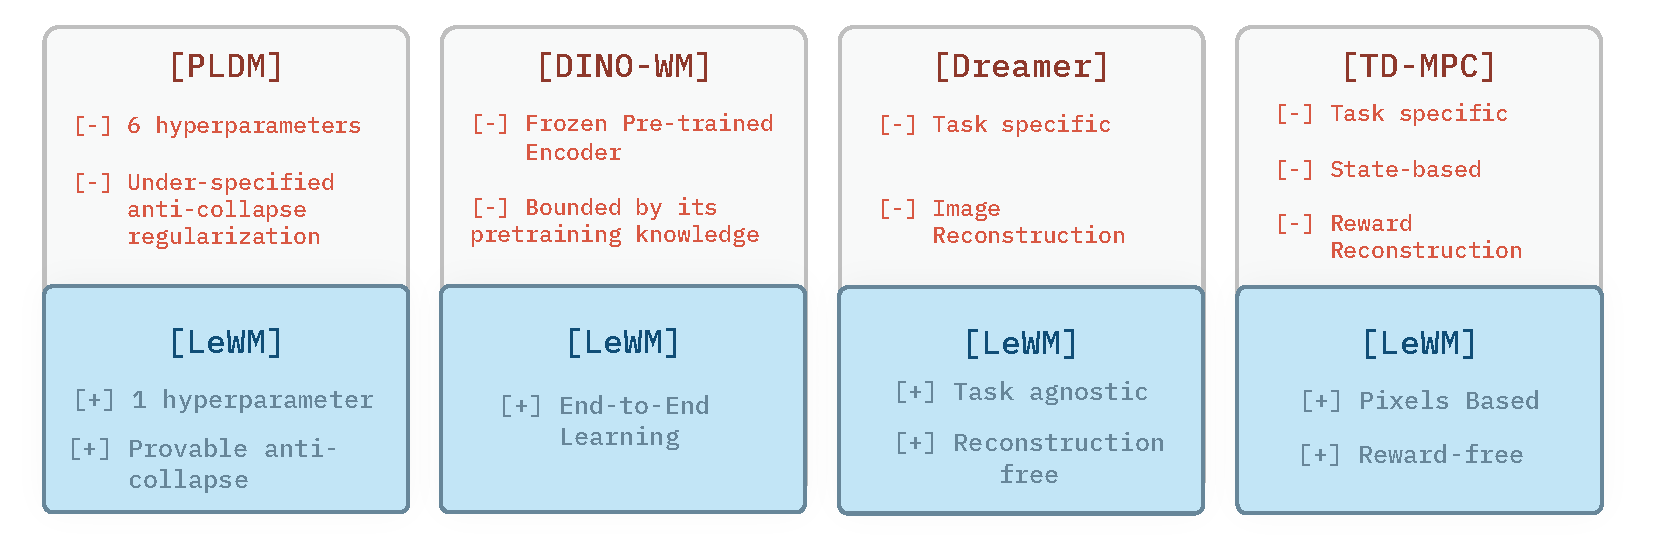
\includegraphics[width=\linewidth]{figs/wms.pdf}
    \caption{\small \textbf{Characteristics of latent world model approaches.} Methods are grouped by training paradigm. \textit{End-to-end} methods (PLDM) learn both the encoder and predictor jointly from pixels without relying on pre-trained representations or heuristic tricks such as stop-gradient or exponential moving averages, but require many hyperparameters and lack formal collapse guarantees. \textit{Foundation-based} methods (DINO-WM) avoid collapse by freezing a pre-trained foundation vision encoder, forgoing end-to-end learning. \textit{Task-specific} methods (Dreamer, TD-MPC) require reward signals or privileged state access during training. LeWM addresses the limitations of each category: it is end-to-end, task-agnostic, pixel-based, reconstruction- and reward-free, and requires only a single hyperparameter with provable anti-collapse guarantees.}
    \label{fig:wm}
\end{figure}


A central goal of artificial intelligence is to develop agents that acquire skills across diverse tasks and environments using a single, unified learning paradigm—one that operates directly from sensory inputs of its surroundings--without hand-engineered state representations or domain-specific calibration. Vision is ideally suited for this aim: cameras are inexpensive and scalable, and learning from pixels enables fully end-to-end training from raw sensory input to action \cite{levine2016end}.
World Models (WMs) are a powerful family of methods \cite{ha2018world} that learn to predict the consequences of actions in the environment. When successful, WMs allows agents to plan and to improve themselves solely form their model of the world, i.e., in imagination space. This is particularly valuable in the offline setting, where agents must learn from fixed datasets without environment interaction—leveraging the model to generate synthetic experience and evaluate counterfactual action sequences \cite{micheli2023transformers, hafner2025dreamerv4}.

A recent popular approach for learning world models is the Joint Embedding Predictive Architecture (JEPA)~\cite{lecun2022path}. Instead of attempting to model every aspect of the environment, JEPA focuses on capturing the most relevant features needed to predict future states. Concretely, JEPA learns to encode observations into a compact, low-dimensional latent space and models temporal dynamics by predicting the latent representation of future observations.

However, despite their conceptual simplicity, existing JEPA methods are highly prone to collapse. In this failure mode, the model maps all inputs to nearly identical representations to trivially satisfy the temporal prediction objective leading to unusable representations. Preventing collapse is therefore one of the central challenges in training JEPA models. Many influential works have proposed methods to address this issue. Yet, these approaches typically rely on heuristic regularization, multi-objective loss functions, external sources of information, or architectural simplifications such as pre-trained encoders. In practice, these strategies often introduce additional instability or significantly increase training complexity.

To overcome these limitations, we propose LeWorldModel (LeWM), the first method to learn a stable JEPA end-to-end from raw pixels without heuristic, principled, and simple (cf. Fig \ref{fig:wm}). Furthermore, LeWM can be trained on a single GPU, lowering the barrier to entry for research. We evaluate LeWM across a diverse set of manipulation, navigation, and locomotion tasks in both 2D and 3D environments. In addition, we probe its intuitive physical understanding through targeted probing and surprise-quantification evaluations in latent space. Overall, our key findings and contributions are:

\begin{itemize}
    \item We propose an end-to-end JEPA method for learning a latent world model from raw pixels on a single GPU. The method relies on a simple and stable two-term objective that remains robust across architectures and hyperparameter choices, while enabling efficient logarithmic-time hyperparameter search.
    \item LeWM achieves strong control performance across diverse 2D and 3D tasks with a compact 15M-parameter model, surpassing existing end-to-end JEPA-based approach while remaining competitive with foundation-model-based world models at substantially lower cost, enabling planning up to $48\times$ faster.
    \item We evaluate physical understanding in the latent space through probing of physical quantities and a violation-of-expectation test for detecting unphysical trajectories.
\end{itemize}


